\section{tasks::task Class Reference}
\label{classtasks_1_1task}\index{tasks::task@{tasks::task}}
Inheritance diagram for tasks::task::\begin{figure}[H]
\begin{center}
\leavevmode
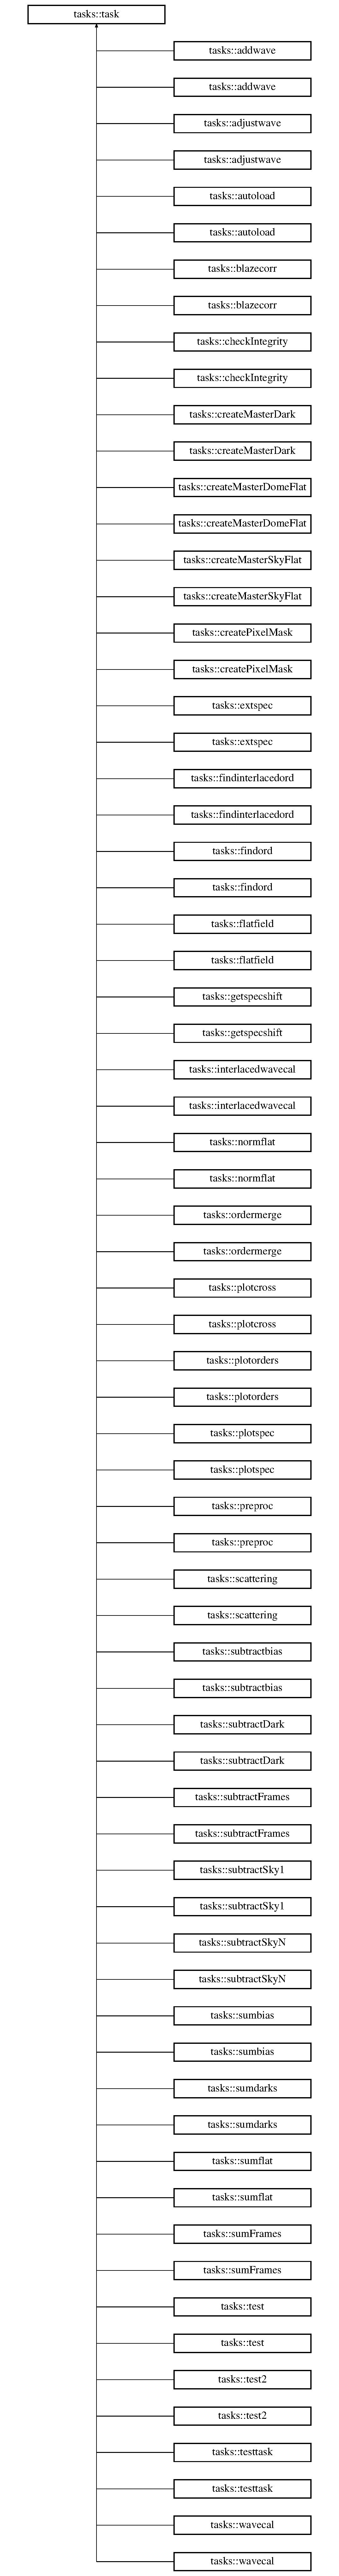
\includegraphics[height=12cm]{classtasks_1_1task}
\end{center}
\end{figure}
\subsection*{Public Member Functions}
\begin{CompactItemize}
\item 
def \textbf{\_\-\_\-init\_\-\_\-}\label{classtasks_1_1task_6c6d93968e1985dcdeb9a427e5887caf}

\item 
def \textbf{\_\-\_\-init\_\-\_\-}\label{classtasks_1_1task_6c6d93968e1985dcdeb9a427e5887caf}

\end{CompactItemize}
\subsection*{Static Public Attributes}
\begin{CompactItemize}
\item 
string \textbf{name} = 'undefined'\label{classtasks_1_1task_9d5daece96641b7ccc3b23b081699b6d}

\item 
string \textbf{button\-Text} = 'Not defined'\label{classtasks_1_1task_47c74a10937d34df8c3557b816f8f277}

\item 
\textbf{suffix} = None\label{classtasks_1_1task_6392c45806636706521d0d44d8bf9201}

\item 
int \textbf{inthread} = 1\label{classtasks_1_1task_a36a990ce7efee7b6e78f06c5b107675}

\item 
int \textbf{output} = 1\label{classtasks_1_1task_f090c423ef95574cf59a5349659a63cc}

\item 
list \textbf{prereq} = [$\,$]\label{classtasks_1_1task_224e6683b391e12fce9ff0882e5e012b}

\end{CompactItemize}


\subsection{Detailed Description}


\footnotesize\begin{verbatim}Description not given\end{verbatim}
\normalsize
 



The documentation for this class was generated from the following files:\begin{CompactItemize}
\item 
old/PANICtool-1.0/tasks.py\item 
old/tasks.py\end{CompactItemize}
